\underbar{\textbf{\large Ejercicio 1:}} Dado el siguiente diagrama, defina las clases que aparecen escribiendo los miembros imprescindibles para implementar las relaciones dadas:
\begin{figure}[h]
  \begin{center}
    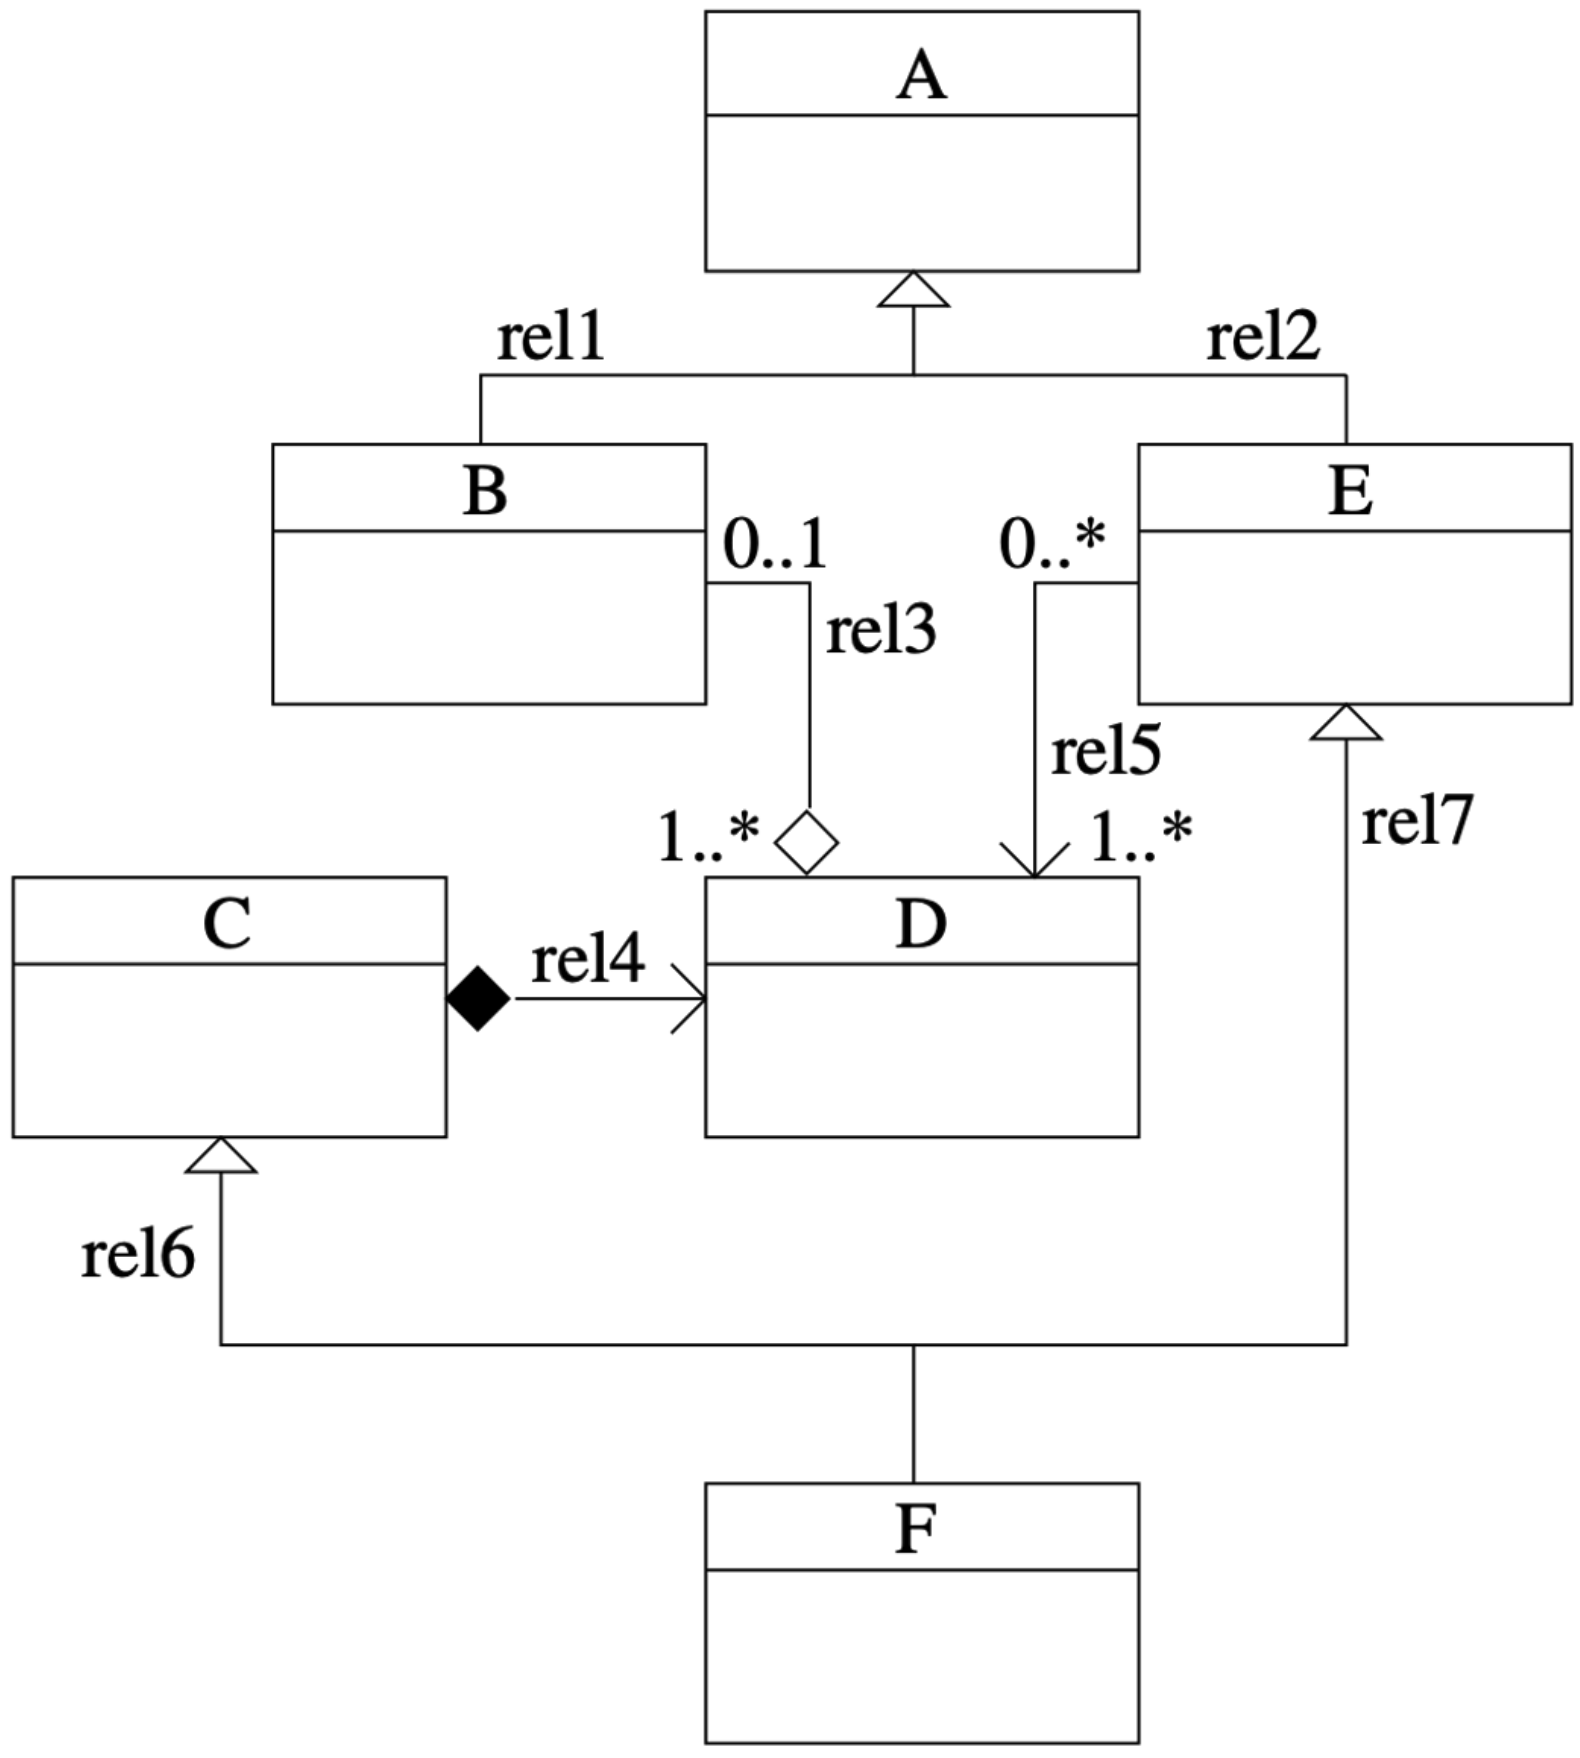
\includegraphics[width=0.4\textwidth]{assets/Mayo2008_1.png}
  \end{center}
  \caption{Diagrama de clases del ejercicio}
\end{figure}
\begin{minted}[breaklines]{C++}
class A{//...};
class B : public A{
  public:
    B(A& a):A(a){} //rel1
};
class C : private D{}; //rel4, composición 1-1, herencia privada
class D{
  public:
    //relacion rel3 (agregación con B), solo conoce el agregado
    void rel3(B&)noexcept;
    const B& getBs()const noexcept;
  private:
    B bs_; //rel3
};

class E : public A{ //rel1
  public:
    //Alias de la relacion con D, es unidireccional
    //multiplicidad 1-muchos, la existencia depende
    E(D& d,A& a):A(a){
      ds_.insert(&d);
    }
    typedef std::set<D*>Ds;
    void setD(D& )noexcept;
    const Ds& getDs()const noexcept;
  private:
    Ds ds_;
};

class F : public C, public E{
  public:
    F(C& c, E& e):C(c),E(e){}
};
\end{minted}

\underbar{\textbf{\large Ejercicio 2:}} Dada las siguientes definiciones de las clases:

\begin{lstlisting}[frame = single]
using namespace std;

class X{
  public:
    X(string s = "por omision"){
      cout<<"Constructor de X: "<<s<<endl;
      }
};

class A{
    X x;
  public:
    A():x("A"){cout<<"Constructor de A"<<endl;}
    void f(){cout<<"Metodo f() de A"<<endl;}
};
class B : virtual public A{
    X x;
  public:
    B() {cout<<"Constructor de B"<<endl;}
    void f(){cout<<"Metodo f() de B"<<endl;}
};
class C : virtual public A{
    X x;
  public:
    C(){cout<<"Constructor de C"<<endl;}
    void f(){cout<<"Metodo f() de C"<<endl;}
};
class D : public B, public C{
    X x;
  public:
    D(): x("D"){cout<<"Constructor de D"<<endl;}
};
\end{lstlisting}
\textbf{\large Apartado a) ¿Cuántos atributos y métodos tiene la clase D?}

La clase D tiene 4 atributos y tiene 3 métodos f().

\textbf{\large Apartado b) ¿Hay algún miembro duplicado?}

Gracias a la herencia virtual solucionamos el problema de la ambigüedad, haciendo que no hayan miembros repetidos.

\textbf{\large Apartado c) ¿Cómo se accede a cada uno de los miembros?}
No podemos acceder a los atributos ya que estos son privados, pero podemos acceder a los métodos de la manera → \texttt{d.D::f()}, \texttt{d.B::f()} y \texttt{d.A::f()}.
\newpage
A continuación, considere el siguiente programa que incluye las definiciones:

\textbf{\large Apartado d) Diga si hay ambigüedades en la función main().\\En tal caso, resuélvalas.}
\begin{lstlisting}[frame=single]
int main(){
  A *pa;
  B *pb;
  D d, *pd;

  pd = &d; //OK, apuntamos a un objeto del mismo tipo
  pa = &d; //OK, conversion de puntero de A - D implicitamente
  pa -> f(); //OK, metodo f() de A (A no polimorfica, se mira tipo puntero)
  pb = &d; //OK, conversion de puntero de B - D implicitamente
  pb -> f(); //OK, metodo f() de B (B no polimorfica, se mira tipo puntero)
  // d= *pa; //ERROR, conversion implicita de objetos hacia abajo.
  pd = (D*)pb; //OK, conversion correcta explicita de B - D
  pd -> B::f(); //OK, metodo f() de B (resolucion de ambito)
  d.C::f(); //OK, metodo f() de C (resolucion de ambito)
  return 0;
}
\end{lstlisting}

Vemos que obtenemos un error en la linea \texttt{d = *pa} ya que estamos haciendo una conversión implícita hacia abajo, no podemos asignar un objeto de tipo A a uno de tipo D de forma implícita.

\textbf{\large Apartado f) Diga lo que imprimiría el programa una vez subsanadas las ambigüedades y los demás errores.}
\begin{figure}[h]
  \begin{center}
    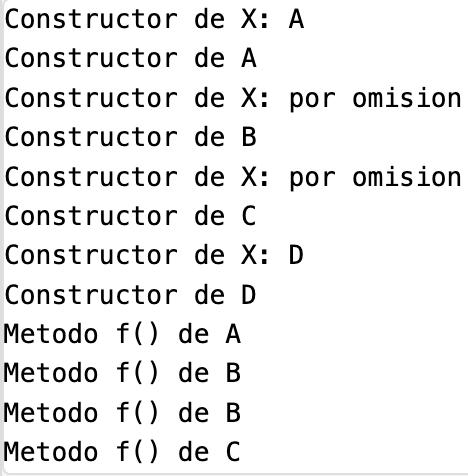
\includegraphics[width=0.5\textwidth]{assets/Mayo2008_2_1.jpeg}
  \end{center}
  Esto obtenemos si omitimos el error comentado anteriormente.
\end{figure}
